\PassOptionsToPackage{unicode,pdfusetitle}{hyperref}
\PassOptionsToPackage{hyphens}{url}
\PassOptionsToPackage{dvipsnames,svgnames,x11names}{xcolor}

\documentclass[10pt,ignorenonframetext]{beamer}

\usepackage{lmodern}
\usepackage{amssymb,amsmath,mathtools,amsthm}
\usepackage[T1]{fontenc}
\usepackage[utf8]{inputenc}
\usepackage{textcomp} % provide euro and other symbols

\usepackage{pgfpages}

\usepackage{multirow}
\usepackage{csvsimple}
\usepackage{siunitx}

% prevent slide breaks in the middle of a paragraph
\widowpenalties 1 10000
\raggedbottom

% Use upquote if available, for straight quotes in verbatim environments
\usepackage{upquote}
\usepackage[]{microtype}
\UseMicrotypeSet[protrusion]{basicmath} % disable protrusion for tt fonts

\usepackage{xcolor}
\usepackage{xurl} % add URL line breaks if available
\usepackage{bookmark}
\usepackage{hyperref}
\hypersetup{%
  colorlinks = true,
  linkcolor  = DarkSlateBlue,
  filecolor  = DarkSlateBlue,
  citecolor  = Orange4,
  urlcolor   = DarkSlateBlue
}

% tikz and pgfplots stuff
\usepackage{tikz}
\usetikzlibrary{arrows,shapes,positioning,intersections}
\usepackage{pgfplots}
\usepgfplotslibrary{external,colormaps}
\pgfplotsset{width=7cm,compat=1.11}
%\tikzexternalize

%\usepackage{subfig}
\usepackage{subcaption}
\usepackage{algorithm,algpseudocode}
\usepackage{booktabs}

% bibliography
\usepackage[citestyle=authoryear]{biblatex}
\addbibresource{references.bib}

\newif\ifbibliography
\setlength{\emergencystretch}{3em} % prevent overfull lines
\setcounter{secnumdepth}{-\maxdimen} % remove section numbering

\AtBeginPart{\frame{\partpage}}
\AtBeginSection{\ifbibliography\else\frame{\sectionpage}\fi}
\AtBeginSubsection{\frame{\subsectionpage}}

\usetheme{boxes}
\usecolortheme{beaver}
\usefonttheme{professionalfonts}
\usefonttheme{structurebold}
\setbeamertemplate{footline}[frame number]
\setbeamertemplate{caption}[numbered]
\setbeamertemplate{caption label separator}{: }
\setbeamercolor{caption name}{fg=normal text.fg}
\setbeamertemplate{itemize item}{\(\bullet\)}
\setbeamertemplate{itemize subitem}{\(\circ\)}
\setbeamertemplate{itemize subsubitem}{\textendash}
\setbeamerfont{frametitle}{size=\large}
\setbeamerfont{framesubtitle}{size=\small}
% \setbeamertemplate{headline}{\vskip4ex}
\beamertemplatenavigationsymbolsempty

% operators
\DeclareMathOperator*{\argmax}{arg\,max}
\DeclareMathOperator*{\argmin}{arg\,min}
\DeclareMathOperator{\sign}{sign}
\DeclareMathOperator{\E}{E}
\DeclareMathOperator{\var}{Var}

% macros
\newcommand{\pkg}[1]{\textsf{#1}}
\renewcommand{\vec}[1]{\bm{#1}}
\newcommand{\mat}[1]{\bm{#1}}
\newcommand{\du}{\mathrm{d}}



% title block
\title{The Hessian Screening Rule}
\subtitle{NeurIPS 2022}
\author[shortname]{\texorpdfstring{\alert{Johan Larsson}}{Johan Larsson} \and Jonas Wallin}
\institute{Department of Statistics, Lund University}
\date{\today}
\titlegraphic{\includegraphics{figures/logo.pdf}}

\begin{document}

\frame[noframenumbering,plain]{\titlepage}

% \begin{frame}{This Talk}
%   In this talk I will present a highly efficient screening rule for the Lasso    
% \end{frame}

\begin{frame}{The Lasso}
  A type of penalized regression, represented by the following
  convex optimization problem:
  \[
    \operatorname*{minimize}_{\beta \in \mathbb{R}^p}
    \left\{
      f(\beta) + \lambda \lVert \beta \rVert_1.
    \right\}
  \]
  where \(f(\beta)\) is smooth and convex. \medskip

  \begin{columns}[T]
    \begin{column}{0.45\linewidth}
      \(f(\beta) = \frac 1 2 \lVert y - X\beta\rVert_2^2\)
      leads to the ordinary lasso. \medskip

      \(\lambda\) is a hyperparameter that controls the level of
      \alert{penalization}. \medskip

      \(\hat\beta(\lambda)\) is the solution to this problem for a given
      \(\lambda.\)

    \end{column}
    \begin{column}{0.45\linewidth}
      \begin{figure}
        \centering
        \pgfplotsset{width=6cm,height=6cm}
        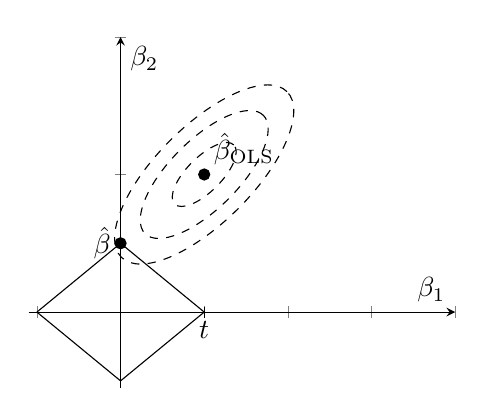
\begin{tikzpicture}
\begin{axis}[
    xlabel = \(\beta_1\),
    ylabel = \(\beta_2\),
    ymin = -1.1,
    ymax = 4,
    xmin = -1.1,
    xmax = 4,
    axis lines = center,
    yticklabels={,,},
    xticklabels={,,}
]
\draw[dashed, rotate around={45:(1,2)}] (1,2) ellipse (0.5 and 0.25);
\draw[dashed, rotate around={45:(1,2)}] (1,2) ellipse (1 and 0.5);
\draw[dashed, rotate around={45:(1,2)}] (1,2) ellipse (1.4 and 0.7);

\addplot[]
    coordinates {
    	(-1,0)
    	(0,1)
    	(1,0)
    	(0,-1)
    	(-1,0)
    };
    
\addplot [only marks, mark=*] coordinates {(1,2)};
\node [above right,black] at (1,2) {\(\hat\beta_\text{OLS}\)};

\addplot [only marks, mark=*] coordinates { (0,1) };
\node [left] at (0,1) {$\hat\beta$};

\addplot [only marks, mark = |] coordinates { (1, 0) };
\node [below] at (1,0) {\(t\)};
\end{axis}
\end{tikzpicture}
      \end{figure}
    \end{column}
  \end{columns}
\end{frame}

\begin{frame}{The Lasso Path}
  \begin{columns}[T, onlytextwidth]
    \begin{column}{0.5\linewidth}

      Solving the lasso for \(\lambda \in [0, \lambda_\text{max})\), with
      \[\lambda_\text{max} \coloneqq \max \big\{ \lambda \in \mathbb{R}^+ \mid
        \hat\beta(\lambda) = 0\big\},\]
      traces the set of all solutions for the lasso. \medskip

      The lasso path is \alert{piece-wise linear} with breaks wherever the active set changes. \medskip

      \alert{The active set}: \[
        \{i : |\beta_i| \neq 0\}.
      \]


    \end{column}
    \begin{column}{0.5\linewidth}
      \begin{figure}
        \includegraphics{figures/lasso-path}
        \caption{The lasso path for an example of the ordinary lasso}
      \end{figure}
    \end{column}
  \end{columns}

\end{frame}

\begin{frame}{Picking \(\lambda\)}

  \begin{block}{The Problem}
    Typically don't know the optimal value for
    \(\lambda\). To tackle this, we use cross-validation to tune for
    \(\lambda\).
  \end{block}

  \pause

  \begin{block}{Grid Search}
    For \(p \gg n\), the standard procedure is to create a
    grid of \(\lambda\)s and solve the lasso numerically.
  \end{block}

  \medskip

  \pause

  But this is computationally demanding when \(p\) is large.

\end{frame}

\section{Screening Rules}

\begin{frame}{Feature Screening}
  \begin{block}{Motivation}
    Many solutions along the regularization path are \alert{sparse},
    especially if \(p \gg n\) since the number of active features cannot exceed \(\min(n, p)\).
  \end{block}

  \pause

  \begin{block}{Basic Idea}
    Say that we are at step \(k\) on the lasso path and are about to solve for
    step \(k + 1\). \medskip

    Intuitively, information at \(k\) should tell us something
    about which features are going to be active at step \(k + 1\). \medskip

    The idea is to use this information to \alert{discard} a subset of the
    features and fit the model to a smaller set of features---the screened
    set.
  \end{block}
\end{frame}


% \begin{frame}{Types of Screening Rules}
%   \begin{block}{Safe Rules}
%     Certifies that discarded features are inactive at the optimum.
%   \end{block}
%   \pause
%   \begin{block}{Heuristic (Un-Safe) Rules}
%     No guarantees! Can result in \alert{violations}: discarding features that
%     are active at the optimum. \medskip

%     Need post-optimization checks of optimality
%     conditions. \medskip

%     Checking the optimality conditions can be costly.
%   \end{block}
% \end{frame}

% \begin{frame}{Optimality Conditions}
%   \(\beta\) is a solution to the lasso problem if it satisfies the stationarity
%   criterion
%   \[
%     \boldsymbol{0} \in \nabla f(\beta) + \lambda \partial
%   \]
%   where \(\partial\) is the subdifferential of \(\lVert \beta \rVert_1\),
%   defined as
%   \[
%     \partial_j \in
%     \begin{cases}
%       \{\sign(\beta_j)\} & \text{if } \beta_j \neq 0, \\
%       [-1,1]             & \text{otherwise.}
%     \end{cases}
%   \]
%   \pause
%   This means that
%   \[
%     |\nabla f(\beta)_j| < \lambda \implies \hat\beta_j = 0.
%   \]
%   Of course, we don't know \(\nabla f(\beta)\) prior to solving the problem.

%   % TODO: insert subdifferential plot
% \end{frame}

\begin{frame}{The Gradient Perspective of the Path}
  \begin{figure}
    \input{figures/lasso-path-gradient.tikz}
    \caption{The gradient vector along the lasso path}
  \end{figure}
\end{frame}

\begin{frame}{Screening Rules Seen As Gradient Estimates}
  Let \(c(\lambda) \coloneqq -\nabla f(\beta(\lambda))\)
  be the so-called \alert{correlation} vector.

  \medskip

  \(\boldsymbol{0} \in \nabla f(\beta)
  + \lambda \partial\) suggests a simple template for a screening rule:
  \begin{enumerate}
    \item Replace \(c\) with an estimate \(\tilde c\).
    \item If \(|\tilde c_j| < \lambda\), discard feature \(j\).
  \end{enumerate}

  \medskip

  If \(\tilde c\) is accurate and not too conservative, we
  have a useful rule.
\end{frame}

% \begin{frame}{The Strong Rule}
%   The Strong Rule gradient estimate is
%   \[
%     \tilde c^S(\lambda_{k+1}) =
%     \underbrace{c(\lambda_k)}_\text{previous gradient} +
%     \underbrace{(\lambda_k - \lambda_{k+1})\sign(c(\lambda_k))}_\text{unit
%       slope
%       bound}.
%   \]
%   \begin{columns}[T]
%     \begin{column}{0.45\linewidth}
%       \alert{Simple idea}\\
%       Assume that the slope of the gradient is bounded by one (the
%       unit slope bound)~\parencite{tibshirani2012}. \medskip


%       Unfortunately, the Strong Rule is conservative when feature are correlated. \medskip
%     \end{column}
%     \begin{column}{0.45\linewidth}
%       \centering
%       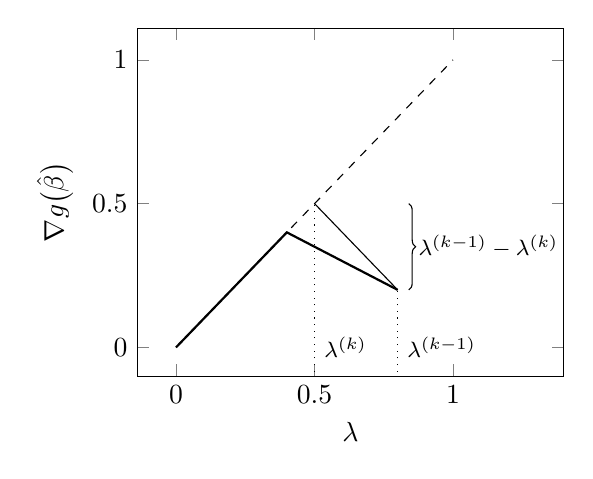
\begin{tikzpicture}
\begin{axis}[
    ylabel = \(\nabla g\big(\hat\beta\big)\),
    xlabel = \(\lambda\),
    xmax = 1.4,
    ymin = -0.1,
    width = 7cm,
    height = 6cm
]
\addplot[style = dashed]
    coordinates {
        (0,0)
        (1,1)
    };
\addplot[]
    coordinates {
        (0.8,0.2)
        (0.5,0.5)
    };
\addplot[thick]
    coordinates {
        (0.8,0.2)
        (0.4,0.4)
        (0,0)
    };
\draw [decorate,decoration={brace},xshift=4pt]
(0.8,0.5) -- (0.8,0.2)node [right,black,midway] {\footnotesize
$\lambda^{(k-1)}-\lambda^{(k)}$};

\addplot[style=dotted]
    coordinates {
        (0.5,-0.2)
        (0.5,0.5)
    };
\addplot[style=dotted]
    coordinates {
        (0.8,-0.2)
        (0.8,0.2)
    };
\node [right] at (0.5,0) {\footnotesize$\lambda^{(k)}$};
\node [right] at (0.8,0) {\footnotesize$\lambda^{(k-1)}$};
\end{axis}
\end{tikzpicture}
%       % \caption{The unit slope bound}
%     \end{column}
%   \end{columns}
% \end{frame}

% \begin{frame}{The Working Set Algorithm}
%   The Strong Rule is conservative when features are correlated. \medskip

%   A better alternative is to use the features that have
%   \alert{ever been active} as a screened set and then
%   \begin{enumerate}
%     \item fit the lasso on the features in the screened set,
%     \item check the optimality conditions in the strong set, and then
%     \item check the optimality conditions for all features.
%   \end{enumerate}
%   Whenever we encounter violations (in step 2 or 3), go back to step 1 and
%   repeat.
% \end{frame}

\section{The Hessian Screening Rule}

\begin{frame}{The Ordinary Lasso}
  We now focus on the ordinary lasso, \(\ell_1\)-regularized least
  squares:
  \[
    f(\beta) = \frac 1 2 \lVert y - X\beta \rVert_2^2
  \]
  and
  \[
    \nabla f(\beta) = X^T(X\beta - y).
  \]
  \pause
  It turns out that we can express the solution as a function of
  \(\lambda\):
  \begin{equation*}
    \label{eq:solution}
    \hat\beta(\lambda) = \big({X_\mathcal{A}}^TX_\mathcal{A}\big)^{-1}
    \big({X_\mathcal{A}}^Ty - \lambda \sign(\hat\beta_\mathcal{A})\big).
  \end{equation*}
  \pause
  This expression holds for an interval \([\lambda_k,\lambda_{k+1}]\) in which
  no changes occur in the active set, which means we can retrieve any solution
  in this range via
  \begin{equation*}
    \hat\beta(\lambda_{k+1})_\mathcal{A} =
    \hat\beta(\lambda_k)_\mathcal{A} -
    (\lambda_k - \lambda_{k+1})\big({X_\mathcal{A}}^TX_\mathcal{A}\big)^{-1}
    \sign\big(\hat\beta(\lambda_k)_\mathcal{A}\big).
  \end{equation*}
\end{frame}

\begin{frame}{The Hessian Screening Rule}
  Take this expression and stick it into the gradient at step \(k +
  1\):
  \begin{equation*}
    \begin{aligned}
      \tilde c^H(\lambda_{k+1})
       & = -\nabla f\big(\hat\beta(\lambda_{k+1})_\mathcal{A}\big)       \\
       & = c(\lambda_k) + (\lambda_{k+1} - \lambda_k)X^T {X_\mathcal{A}}
      \big({X_\mathcal{A}}^T{X_\mathcal{A}}\big)^{-1}
      \sign\big(\hat\beta(\lambda_k)_\mathcal{A}\big),
    \end{aligned}
  \end{equation*}
  which is the basic form of our screening rule: \alert{The Hessian Screening
    Rule}. \medskip

  Note that this is an exact expression for the correlation vector (negative
  gradient) at step \(k+1\) if the activate set has remained unchanged.\medskip

  The Hessian Screening Rule is a heuristic (un-safe) rule, so it needs safe-guarding
  in order to avoid discarding active features.
\end{frame}

\begin{frame}{The Hessian and Strong Screening Rules}
  \begin{figure}
    \input{figures/estimate-comp.tikz}
    \caption{Conceptual comparison of screening rules}
  \end{figure}
\end{frame}

% \begin{frame}{Tweaks}
%   \begin{block}{Avoiding Expensive Inner Products}
%     The expression
%     \begin{equation*}
%       \hat c^H(\lambda_{k+1})
%       = c(\lambda_k) + (\lambda_{k+1} - \lambda_k)X^T {X_\mathcal{A}}
%       \big({X_\mathcal{A}}^T{X_\mathcal{A}}\big)^{-1}
%       \sign\big(\hat\beta(\lambda_k)_\mathcal{A}\big),
%     \end{equation*}
%     involves an expensive inner product with the full design matrix.
%     \medskip

%     Instead, we replace \(X\) with the columns indexed by the strong rule.
%   \end{block}

%   \pause

%   \begin{block}{Upwards Shift}
%     We need some upwards bias on the estimate or else risk excessive numbers of
%     violations. We add a fraction \(\gamma\) of the unit bound\footnote{We've
%       set \(\gamma = 0.01\) in our simulations, which has worked very well.}.
%   \end{block}

% \end{frame}

% \begin{frame}{Warm Starts}
%   The availability of the Hessian inverse enables a better warm start:
%   \[
%     \hat\beta(\lambda_{k+1})_\mathcal{A} \coloneqq
%     \hat\beta(\lambda_k)_\mathcal{A} +
%     (\lambda_k - \lambda_{k+1}) \big({X_\mathcal{A}}^T{X_\mathcal{A}}\big)^{-1}
%     \sign\big(\hat\beta(\lambda_k)_\mathcal{A}\big)
%   \]
%   \pause
%   \begin{figure}
%     \centering
%     \includegraphics{figures/hessian-warm-starts}
%     \caption{Number of passes of coordinate descent for two datasets
%       using either Hessian warm
%       starts or standard warm starts.}
%   \end{figure}
% \end{frame}

% \begin{frame}{Updating the Hessian}
%   Computing the Hessian and its inverse naively is expensive:
%   \(\mathcal{O}(|\mathcal{A}|^3 + |\mathcal{A}|^2n)\).

%   \medskip

%   Fortunately, we can sweep columns of the Hessian and inverse in our out,
%   yielding complexity
%   \begin{itemize}
%     \item \(\mathcal{O}(|\mathcal{D}|^2n + n|\mathcal{D}||\mathcal{E}| +
%           |\mathcal{D}^2||\mathcal{E}| + |\mathcal{D}|^3)\) when
%           augmenting the Hessian and
%     \item \(\mathcal{O}(|\mathcal{C}|^3 + |\mathcal{C}|^2|\mathcal{E}| +
%           |\mathcal{C}||\mathcal{E}|^2)\) when reducing it,
%   \end{itemize}
%   where
%   \begin{itemize}
%     \item \(\mathcal{C} = \mathcal{A}_{k-1} \setminus \mathcal{A}_k\)
%           (to-be deactivated),
%     \item \(\mathcal{D} = \mathcal{A}_k \setminus \mathcal{A}_{k-1}\)
%           (to-be activated), and
%     \item \(\mathcal{E} = \mathcal{A}_k \cap \mathcal{A}_{k-1}\)
%           (still activate).
%   \end{itemize}
% \end{frame}

% \begin{frame}{General Loss Functions}

%   The rule can be extended to many other loss functions as long as they are
%   twice-differentiable, but note that
%   \begin{itemize}
%     \item the gradient estimate now involves a matrix of weights---for logistic
%           regression a diagonal matrix,
%     \item the lasso path is no longer piece-wise linear, and
%     \item updating the Hessian is no longer cheap.
%   \end{itemize}
% \end{frame}

\subsection{Results}

\begin{frame}{Setup}
  \begin{itemize}
    \item Rows of the feature matrix i.i.d. from
          \(\mathcal{N}(0,\Sigma)\)
    \item Response generated from \(\mathcal{N}(X\beta,\sigma^2 I)\)
          with
          \(\sigma^2 = \beta^T\Sigma \beta/\text{SNR}\)
    \item \(s\) non-zero coefficients, equally spaced throughout the
          coefficient vector
  \end{itemize}

  \begin{block}{Scenario 1 (Low-Dimensional)}
    \(n = 10\,000\), \(p = 100\), \(s = 5\), and \(\text{SNR} = 1\)
  \end{block}

  \begin{block}{Scenario 2 (High-Dimensional)}
    \(n = 400\), \(p = 40\,000\), \(s = 20\), and \(\text{SNR} = 2\)
  \end{block}

  \medskip

  Code is located at

  \href{https://github.com/jolars/HessianScreening}{\nolinkurl{github.com/jolars/HessianScreening}}
\end{frame}

\begin{frame}{Effectiveness}
  \begin{figure}
    \centering
    \includegraphics{figures/simulateddata-efficiency}
    \caption{
      Number of features screened 
      when fitting a lasso path for \(\ell_1\)-regularized
      least-squares to a design with varying correlation (\(\rho\)),
      \(n = 200\), and \(p = 20000\). The actual number of active
      features at each step across iterations is given as a dashed line.
    }
  \end{figure}
\end{frame}

\begin{frame}{Simulated Data}
  \begin{figure}
    \centering
    \includegraphics{figures/simulateddata-timings}
    \caption{Time to fit a full regularization path for
      \(\ell_1\)-regularized least-squares and logistic regression to
      a design with \(n\) observations, \(p\) features, and pairwise
      correlation between features of \(\rho\). Time is relative to the
      minimal value for each group.}
  \end{figure}
\end{frame}

% \begin{frame}{Real Data: Least-Squares Regression}
%   \begin{table}[hbtp]
%     \caption{
%       Average time to fit a full regularization path of \(\ell_1\)-regularized
%       least-squares regression to real data sets.
%       \label{tab:performance-realdata}}
%     \addtolength{\tabcolsep}{-2pt}
%     \csvreader[
%       tabular={
%           l
%           S[table-format=6.0,round-mode=off]
%           S[table-format=7.0,round-mode=off]
%           S[table-format=1.4,scientific-notation=false,round-precision=2]
%           S[table-format=3.3]
%           S[table-format=3.3]
%           S[table-format=3.3]
%           S[table-format=3.3]
%         },
%       before reading=\scriptsize\centering\sisetup{round-mode=figures,
%         round-precision=3},
%       table head=\toprule & & & & \multicolumn{4}{c}{Time (s)} \\
%       \cmidrule(lr){5-8} Data Set & {\(n\)} & {\(p\)} & {Density} & {Hessian} &
%       {Working} & {Blitz} & {Celer} \\\midrule,
%       table foot=\bottomrule
%     ]%
%     {tables/realdata-timings-gaussian.csv}%
%     {dataset=\dataset, n=\n, p=\p, density=\density, Hessian=\hessian,
%       Working=\working, Blitz=\blitz,
%       Celer=\celer}%
%     {\dataset & \n & \p & \density & \hessian & \working & \blitz & \celer}
%   \end{table}
% \end{frame}

% \begin{frame}{Real Data: Logistic Regression}

%   \begin{table}[hbtp]
%     \caption{
%       Average time to fit a full regularization path of \(\ell_1\)-regularized
%       logistic regression to real data sets.
%       \label{tab:performance-logreg}}
%     \addtolength{\tabcolsep}{-2pt}
%     \csvreader[
%       tabular={
%           l
%           S[table-format=6.0,round-mode=off]
%           S[table-format=7.0,round-mode=off]
%           S[table-format=1.1e-1,scientific-notation=true,round-precision=2]
%           S[table-format=4.3]
%           S[table-format=4.2]
%           S[table-format=4.2]
%           S[table-format=4.2]
%         },
%       before reading=\scriptsize\centering\sisetup{round-mode=figures,
%         round-precision=2},
%       table head=\toprule & & & & \multicolumn{4}{c}{Time (s)} \\
%       \cmidrule(lr){5-8} Data Set & {\(n\)} & {\(p\)} & {Density} & {Hessian} &
%       {Working} & {Blitz} & {Celer} \\\midrule,
%       table foot=\bottomrule
%     ]%
%     {tables/realdata-timings-binomial.csv}%
%     {dataset=\dataset, n=\n, p=\p, density=\density, Hessian=\hessian,
%       Working=\working, Blitz=\blitz,
%       Celer=\celer}%
%     {\dataset & \n & \p & \density & \hessian & \working & \blitz & \celer}
%   \end{table}
% \end{frame}

\begin{frame}{Discussion}
  \begin{itemize}
    \item Simple, intuitive, idea
    \item Performs well in our examples
    \item Handles the highly-correlated case very well
    \item Works for arbitrary loss functions that are twice differentiable
    \item Works for other penalty functions too (SLOPE, MCP, SCAD, Elastic Net)
  \end{itemize}
\end{frame}

% \begin{frame}[allowframebreaks]{References}
%   \bibliographytrue
%   \printbibliography[heading=none]
% \end{frame}

\end{document}
